\chapter{Impact on stakeholders and markets, strategic aspects}

This section starts by analysing an hipotetical situation. Let's supose that we have been hired as by a company with certain business, and we are taken into account as decision making advisors in the area of technology. The company has already made a decision about releasing their key software product under Apache or GPL license, and there is a new meeting to decide which license to choose? And more specifically: \textbf{Which license will attract more companies to collaborate in our business?}\\

We recall that the Apache license type can be classified as permissive, while a GPL as copyleft, each with its own implications. \\

The debate at class started with different approaches, some were inclined to the GPL because it ensured the continuity of the project under the same trend, others by Apache because commercial companies in general have less resistance to such licenses, and others ultimately could not come to any conclusion. Eventually all converged to that there is no formula with calculated results, the choice of a FLOSS license type usually depends on at least the following premises:

\begin{itemize}
\item Desired goal to be obtained with the product
\item Niche market to which the product is intended
\item Presence of the company in the current market
\item Preliminary study of the current market and definition of the possible innovation
\item Among many others
\end{itemize}

Overall we can see that the decision making regarding to Free Software, is not far from other business areas and corresponding analysis, every FLOSS product deserves its specific considerations.

\section{Impact on companies using software and in the production fabric}


One thing is very clear when talking about the economic impact that a business strategy can produce, and it is to be focused from a purely practical point of view. In this sence we watched the video\footnote{http://www.parc.com/event/1092/open-for-business.html} of a lecture at PARC (Palo Alto Research Center) about \textquotedblleft Open for business: Building successful commerce around open source", whose presenter was M\aa rten Mickos, Eucalyptus Systems CEO and ex-CEO of MySQL AB, two successful OSS companies.\\

Some main ideas about the presentation are:

\begin{itemize}
\item A business presentation, not a technical one
\item Make a lot of money with open source is the main goal, because companies are the ones who finances developers and so on, if it requires closed source features or going to the enterprise market, it has to be done in order to sustain
\item For many people is tough talking about FLOSS and business at the same time, because there are mistaken concepts around these topics together
\item FLOSS a better method to produce software (goods), faster (communities), common interest into solve problems (developers), relies over internet (distribution), users are happy with it (customers), but difficult to sell it (companies)
\item When talking from a practical point of view, it is important to differentiate FLOSS from philosophical issues involved
\item Forms of production and distribution are very important, and in this case on intangible assets
\item Maybe FLOSS works because there are people trying to solve their own personal problems over this model, so maybe there is no charity or voluntary at all
\item Important companies such as RedHat or Oracle have inverted lots of money on FLOSS and have shown it is a sustainable model
\item Now when talking about FLOSS, show up words like: serious, commercial and professional
\item Some time ago vendors didn't care about FLOSS, but now customers are demanding it
\item Before quality of software was dictated only by proprietary software companies, but now with FLOSS the quality is in sight of all people
\item The core-business for a company, may be non-core for others, this is a good feature to take advantage of
\item Eventually a company that successfully penetrates with FLOSS a market that was proprietary, tends to enforce the rules
\item FLOSS success vs Commercial success graph, shows the opposite limits that have reached eg. Apache and Microsoft products, as well as products like MySQL DB or Linux kernel occupying the midpoint:
\begin{figure}[h]
\begin{center}
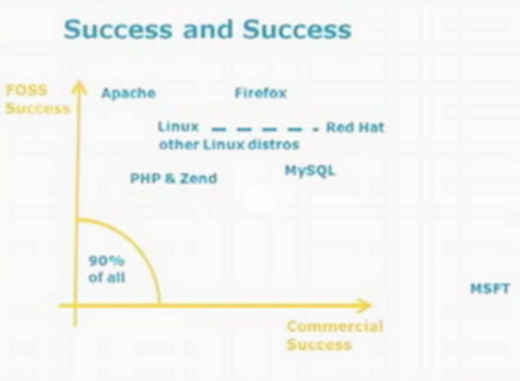
\includegraphics{success}
\caption{FLOSS success vs Commercial success.}
\label{fig:success}
\end{center}
\end{figure}
\end{itemize}


\section{The Economic Motivation of Open Source Software: Stakeholder Perspectives}\label{Part II}

An important consequence that FLOSS brings to the economic market is the emergence of new players in the system. Now there is not only a software manufacturer, channels and customers, but there are also private developers, system integrators and communities that have as much presence as any powerful company in the market of a certain field.\\

From system integrators' perspective, we interpretated a theorical \textquotedblleft IT solutions demand curve"\footnote{http://dirkriehle.com/computer-science/research/2007/computer-2007-article.html}, in which highlights three main factors of IT: hardware, software, and services.\\

\begin{figure}[h]
\begin{center}
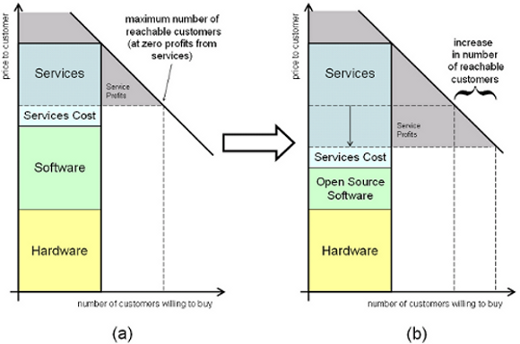
\includegraphics{curve}
\caption{Sales margins and number of customers. (a) The lower price limit determines the customers the system integrator takes on, (b) switching from closed source software to open source software can result in more customers and higher profits.}
\label{fig:curve}
\end{center}
\end{figure}

Based on the fact that the hardware is usually maintained at a stable price, by reducing the costs associated with licensing fees when using FLOSS software, integrators can vary as desired, whether the services provided or the price associated with such services. This represents a great advantage over the use of proprietary software, in the sense that profits areas are more flexible, that is, starting from a certain cost, theoretically can be increased the number of services offered, or could be decreased the price of services in order to attract more customers.\\

Also, depending on whether the product target is massive or not, will require the allocation of a greater or lesser value to recover the investment later. Some examples were mentioned, as for instance:

\begin{itemize}
\item The market for mobile devices, led in part by Google nowadays, is a consequence of the low cost of the software, allowing direct investment almost only into manufacturing hardware, and therefore having a competitive advantage in the price at which the product is offered
\item Android Operating System on any of the tablets from Barnes \& Noble or Samsung, versus Apple's
\end{itemize}

Another concept handled was the cost and the price of intangible assets, who behave differently from tangible ones. From the closed source software vendor perspective a leading software vendor sets a price that maximizes its profits, offering the product to different customers at the same price. Usually most of the investment comes from shipping the first copy of the software. On the other hand in an open source community, given the right license, anyone can set up a company and start selling the software provision, maintenance, and support. Pricing will be based on markup over cost, with a high markup new companies will enter the market, with a low markup companies will leave the market. The first copy of the software is produced in a community without losing the appeal of the product, not necessarily in a cheaper way. Customers benefit from this situation, because they get a much cheaper price compared to proprietary software, and FLOSS vendors also benefit because they displace proprietary products.\\

There is a group of graphics that show a long-run average cost curve for a single software product\footnote{http://dirkriehle.com/computer-science/research/2007/computer-2007-article.html}.

\begin{figure}[h]
\begin{center}
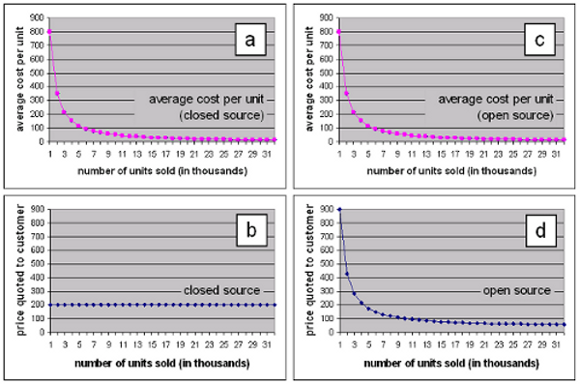
\includegraphics{cost-price}
\caption{Differences in cost and pricing. (a) and (c) show a similar average cost per unit for closed source and open source software, while (b) and (d) indicate the relationship between price and number of units sold for open and closed software.}
\label{fig:cost-price}
\end{center}
\end{figure}

\section{Conclusions}\label{conclusions}

In working process... by Daniel G\'amez.\\
